%----------------------------------------------------------------------------------------
%
%
%
%
%
%----------------------------------------------------------------------------------------



\documentclass[12pt]{article}
\usepackage[dvipsnames]{xcolor}
\usepackage[portuguese]{babel}
\usepackage[utf8x]{inputenc}
\usepackage{amsmath}
\definecolor{coolblack}{rgb}{0.0, 0.18, 0.39}
\usepackage[pdftex,breaklinks,colorlinks=true,citecolor=coolblack,urlcolor=blue,linkcolor=coolblack]{hyperref}
\usepackage{url}
\usepackage{mathtools}
\usepackage{graphicx}
\usepackage[colorinlistoftodos]{todonotes}
\usepackage{float}
\usepackage{indentfirst}
\usepackage{enumitem}
\usepackage[margin=2.4cm]{geometry}
% \usepackage{tikz}
\usepackage{wasysym}
\usepackage{titlesec}
\usepackage{listings}
\usepackage{upquote}
\usepackage{tasks}
\usepackage{pdfpages}
\usepackage[bottom]{footmisc}
\usepackage{dirtytalk}
\usepackage{minted}
\usepackage{subcaption}
\usepackage{fancyhdr}
\usemintedstyle{vs}
\renewcommand{\fcolorbox}[4][]{#4}%}



\newcommand{\HRule}{\rule{\linewidth}{0.5mm}} % Defines a new command for the horizontal lines, change thickness heree


\begin{document}
%----------------------------------------------------------------------------------------
%	HEADING SECTIONS
%----------------------------------------------------------------------------------------
\begin{titlepage}
\pagestyle{fancy}
\renewcommand{\headrulewidth}{0pt}
\renewcommand{\footrulewidth}{0pt}
\setlength\headheight{150.8pt}
\addtolength{\textheight}{-20.0pt}
\chead{
\includegraphics[width=250.0pt]{imgs/UC.jpg}}


\center % Center everything on the page
 %Name of your university/college
\vspace*{1cm}
\textsc{\Large Engenharia Electrotécnica e de Computadores}\\[1.5cm] % Major heading such as course name
\textsc{\LARGE Sensores Inteligentes}\\[0.15cm] % Minor heading such as course title
\textsc{\large Ano Letivo: 2018/2019}\\[2cm]
\textsc{\LARGE \textbf{Mini-Projecto}  }\\[1cm]
\HRule \\[0.6cm]
{ \huge \bfseries Monitorização ambiental}\\[0.3cm]
\HRule \\[0.4cm]
\vspace{2cm}
\textsc{\large PL1 - Grupo 1}\\
\vspace{0.5cm}
\begin{minipage}{0.4\textwidth}
\begin{flushleft} \large
\textsc{Miguel Maranha Tiago}\\
\textsc{Luís Filipe Dias da Cruz}\\
\end{flushleft}
\end{minipage}
\begin{minipage}{0.4\textwidth}
\begin{flushright} \large
\textsc{nr. 2012138309}\\
\textsc{nr. 2011164454}\\
\end{flushright}
\end{minipage}
\thispagestyle{fancy}
\vfill
\end{titlepage}


%%%%%%%%%%%%%%%%%%%%%%%%%%%%%%%%%%%%%%%%%%%%%%%%%%%%%%%%%%%%%%%%%%%%%%%%%%%%%%%%%%%%%%%%%%%%%%%%%%%%
\section{Prefácio}

\textit{Tem-se como objectivo para este trabalho, monitorizar a qualidade do ambiente, mais especificamente de parâmetros relacionados com o Ar. Em determinados espaços interessa analisar e consequentemente controlar as suas variáveis, espaços como Bibliotecas$^{\cite{libs}}$, Estufas$^{\cite{green}}$ ou Salas de seca$^{\cite{dry}}$, etc. Para isso, existem imensos sensores, cada um para um determinado fim ou parâmetro. Para o controlo do sistema foi-nos pedido para usar uma Raspberry PI integrado com MQTT (Message Queuing Telemetry Transport) e fazer uso da linguagem de programação visual Node-RED, no entanto acrescentámos uma PIC24 e um ESP8622, usando o módulo WiFi, para aquisição, tratamento e comunicação dos dados recolhidos. Existem diversas variáveis que se possam considerar interessantes de monitorizar, no entanto depende do ambiente alvo e respectivas necessidades que possam advir do tipo de projecto a realizar. Neste trabalho escolhemos a Temperatura, Humidade, Pressão e Luminosidade.}

%%%%%%%%%%%%%%%%%%%%%%%%%%%%%%%%%%%%%%%%%%%%%%%%%%%%%%%%%%%%%%%%%%%%%%%%%%%%%%%%%%%%%%%%%%%%%%%%%%%%

\section{Introdução}

\par Monitorização ambiental descreve os processos e actividades que caracterizam e monitorizam a qualidade do próprio ambiente. Esta monitorização é usada muitas vezes para avaliações de impacto ambiental, como por exemplo, para observar a pegada humana, e como esta está afectando o meio ambiente.\\
Todas as estratégias e ferramentas utilizadas para este fim têm uma razão de ser, são planeadas e projectadas com vista em analisar o estado de um determinado ambiente e também de estabelecer têndencias ou correlações entre os parâmetros ambientais (temperatura, humidade, etc.). Em todos estes casos, os resultados são revistos e analisados estatisticamente, resultando na maior parte das vezes em relatórios oficiais ou artigos publicados.
Assim, um projecto de monitorização ambiental tem sempre de ser pensado e desenhado tendo em conta a finalidade do mesmo. \\
Na monitorização ambiental em determinadas áreas, como no centro de uma cidade, a qualidade do ambiente é de extrema importância tanto para a sobrevivência do ser Humano como para a subsistência do próprio eco-sistema. Como a qualidade do Solo e da Água, a qualidade do Ar é uma das características fundamentais a ser medidas e faz sentido medir parâmetros que transcrevam sinais de poluição: Particulas de matérias ($PM$), Ozono de baixo nível ($CO$), oxidos de enxofre ($SO_x$), oxidos de nitrogénio ($NO_x$), e chumbo ($Pb$). \\
Este trabalho foca-se em ambientes com maior margem de controlo (Bibliotecas, salas de seca, estufas, etc.), onde se possa não só analisar e tirar respectivas conclusões mas também accionar sistemas externos de maneira a influenciar esse ambiente.

%%%%%%%%%%%%%%%%%%%%%%%%%%%%%%%%%%%%%%%%%%%%%%%%%%%%%%%%%%%%%%%%%%%%%%%%%%%%%%%%%%%%%%%%%%%%%%%%%%%%
\newpage
\subsection{Estado da arte}

\par Sensores de medição ambiental estão dísponíveis no mercado, tanto de forma individual como já implementados em plataformas de medição (figura \ref{fig:aeroplats}), como no caso da AQMesh$^{\cite{aqmesh}}$ que incluí sensores já integrados com o intuito de medir todos os parâmetros relativos com qualidade do ar, ou da Aeroqual $^{\cite{aeroqual}}$ (Ver tabela) que dá ao cliente a hipótese de  as personalizar. No entanto este tipo de plataformas pode ir para além das centenas, até aos milhares de euros, muito devido á sua precisão. \\


\begin{figure}[h!]
  \centering
  \begin{subfigure}[b]{0.5\linewidth}
    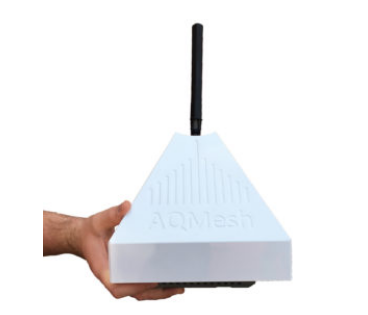
\includegraphics[width=\linewidth]{imgs/aqmesh.png}
    \caption{AQMesh}
  \end{subfigure}
  \begin{subfigure}[b]{0.3\linewidth}
    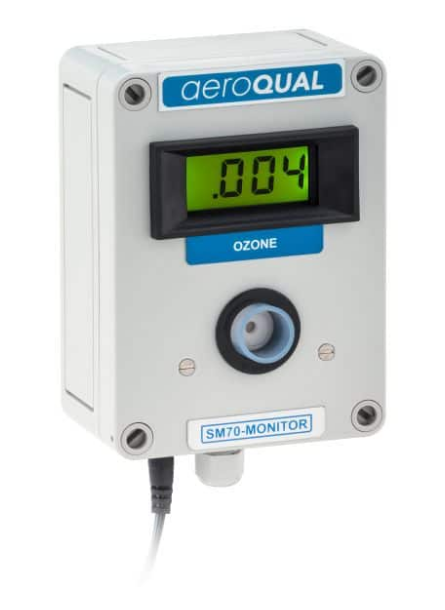
\includegraphics[width=\linewidth]{imgs/airqplat.png}
    \caption{SM70 da Aeroqual}
  \end{subfigure}
  \caption{Exemplo de plataformas sensoriais}
  \label{fig:aeroplats}
\end{figure}

\par Hoje em dia há um leque bastante alargado de sensores por onde escolher, tanto de baixo custo como de consumo, com precisão satisfatória, também dependendo das exigências do utilizador. Alguns dos mais comuns são:
\begin{itemize}
    \item \textbf{BMP280} (Bosch)$^{\cite{BMP280}}$: Sensor de Pressão digital com intervalos de leitura de 300-1100hPa, e $\pm$0.12hPa de precisão, corrente de consumo de 2.7$\mu$A. Preço: $\sim1 EUR$
    \begin{figure}[H]
        \centering
        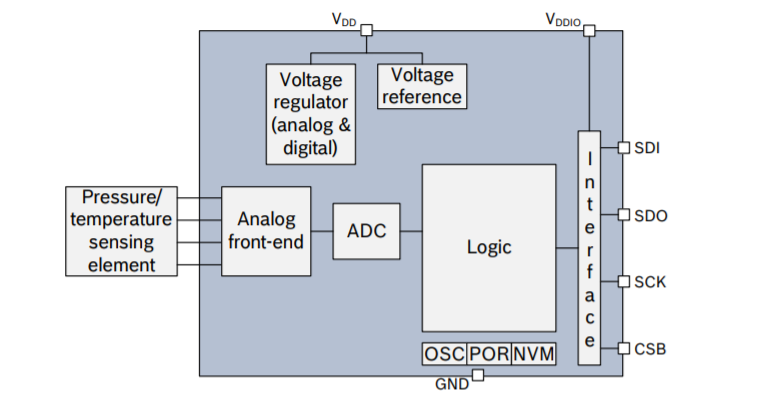
\includegraphics[width=0.6\linewidth]{imgs/bmp280.png}
        \caption{Diagrama de blocos do BMP280}
    \end{figure}
    \item \textbf{HDC1080} (Texas Instruments)$^{\cite{hdc1080}}$: Sensor de Humidade de alta precisão e tem sensor de temperatura integrado, com erro de $\pm0.2\%$ e $\pm$0.2ºC, com $\sim$1$\mu$A corrente de consumo. Preço $\sim2 EUR$
    \begin{figure}[H]
        \centering
        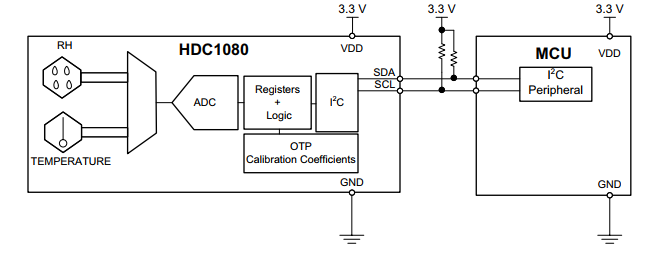
\includegraphics[width=0.6\linewidth]{imgs/hdc1080.png}
        \caption{Diagrama de blocos do HDC1080}
    \end{figure}
    \item \textbf{3SP$\_$NO2$\_$20 C} (Spec Sensors)$^{\cite{no2sensor}}$: Sensor de $NO_2$ com intervalo de medida entre 0-20ppm com erro inferior a 20ppb. Potência entre 10-50$\mu$W. Preço $\sim$20 EUR
    \begin{figure}[H]
        \centering
        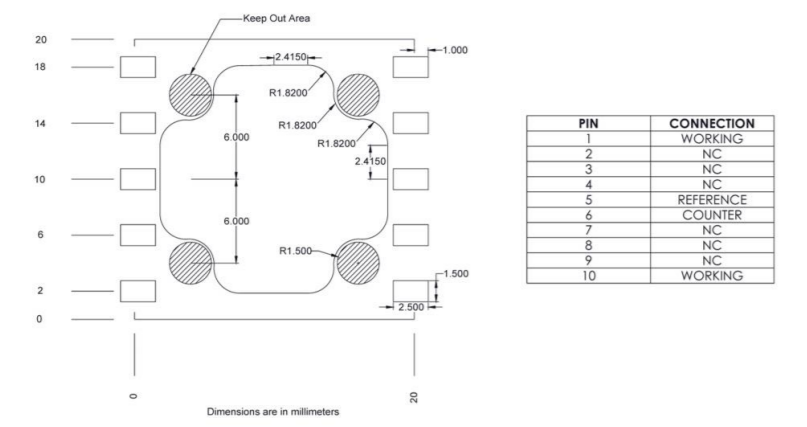
\includegraphics[width=0.6\linewidth]{imgs/no2.png}
        \caption{Diagrama de blocos do 3SP$\_$NO2$\_$20 C}
    \end{figure}
    \item \textbf{GP2Y1010AU0F} (Sharp)$^{\cite{dustsensor}}$: Sensor de particulas óptico, com um díodo emissor de infravermelhos (TX) e um fototransistor (RX) integrados no sensor, detecta a luz reflectida pelas partículas de pó no ar ou até, por exemplo, o fumo provocado pela combustão de um cigarro, consegue distinguir essa diferença através do padrão de pulsos na saída do sensor. Sensibilidade de 0.5$V/(0.1mg/m^3)$ Preço: $\sim$10 EUR
    \begin{figure}[H]
        \centering
        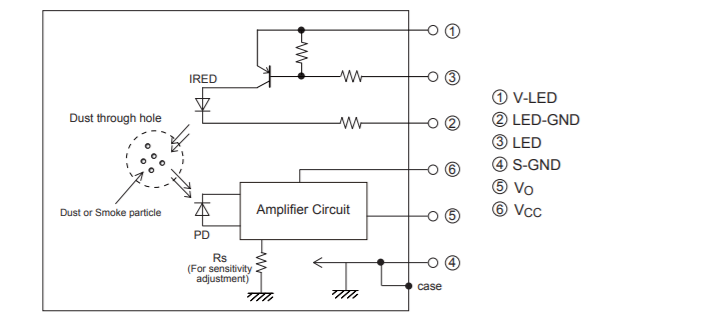
\includegraphics[width=0.6\linewidth]{imgs/dust.png}
        \caption{Diagrama de blocos do GP2Y1010AU0F}
    \end{figure}
\end{itemize}

%%%%%%%%%%%%%%%%%%%%%%%%%%%%%%%%%%%%%%%%%%%%%%%%%%%%%%%%%%%%%%%%%%%%%%%%%%%%%%%%%%%%%%%%%%%%%%%%%%%%

\section{Projecto}

\par Neste capítulo é descrito todo o processo para o desenvolvimento deste projecto e a teoria por detrás do mesmo. Desde a ideia até á implementação.

\subsection{Conceitos Teóricos}
\subsubsection{Resistências dependentes de Luz (LDR)}

\par As resistências são seguramente dos elementos mais comuns em circuitos eléctricos. Regidas pela lei de Ohm (Eq. \ref{eq:Ohm}), em que a corrente é proporcional á diferença de tensão nas extremidades dos seus terminais. 

\begin{equation}\label{eq:Ohm}
    R = \frac{U}{I}
\end{equation}

São usadas para diferentes propósitos, tanto para delimitar a corrente eléctrica como para dividir a tensão ou a corrente através da sua montagem, quer em série ou paralelo, para a dissipação de calor  (Joule's law ref), controlo do ganho, nas últimas décadas como travões eléctricos dissipando energia cinética, etc. Estão comercialmente dísponiveis com valores quase unitários até a grandezas com mais de nove zeros de magnitude.\\
Existem vários tipos de resistências, alguns deles: Resistências de valor fixo, Resistências de valor variável (Termistóres (NTC e PTC) que variam com a mudança de temperatura, Varistores que variam com a mudança de tensão, Resistências magnéticas que variam com a mudança do campo magnético, e foto-resistências que variam com a mudança de luz, também chamadas de LDR's (\textit{Light depending resistor}).\\
Vamos-nos focar neste último caso das foto-resistências.\\

\begin{figure}[h!]
  \centering
  \begin{subfigure}[b]{0.5\linewidth}
    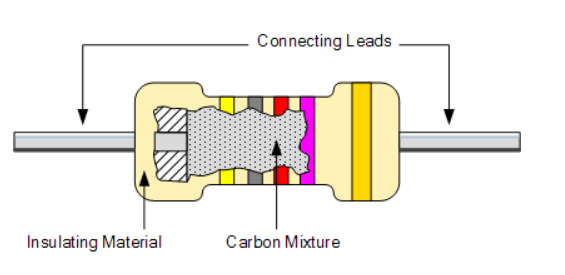
\includegraphics[width=\linewidth]{imgs/resistor.png}
    \caption{Resistência de carbono}
  \end{subfigure}
  \begin{subfigure}[b]{0.3\linewidth}
    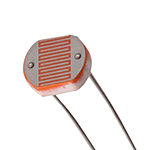
\includegraphics[width=\linewidth]{imgs/photoresistor.png}
    \caption{LDR}
  \end{subfigure}
  \caption{Resistências usadas neste projecto}
  \label{fig:aeroplats}
\end{figure}

As foto-resistências têm a sua resistência nominal bastante alta, tipicamente 1M$\Omega$ e, quando são expostas a luminosidade, a resistência cai agressivamente, até alguns $\Omega$, dependendo da intensidade de luz.\\
Dependendo do material usado nos LDR's, estes podem ser divididos em dois tipos: Intríseco e Extrínseco. Os de primeiro tipo, usam materiais "não dopados", isto é, sem impurezas como o silício ou o germânio. Os fotões que incidem sobre o componente, excitam os electrões presentes na banda de valência e resulta num maior número de electrões livres, que possam transportar corrente e então diminuindo a respectiva resistência. Os LDR's do tipo extrínseco são feitos de materiais dopados com ímpurezas, também chamados de dopantes. Estas ímpurezas criam uma nova banda de energia sobre a banda de valência existente, populando-a com electrões. Estes electrões, por sua vez, precisam de menos energy para fazer a transição para a banda de condução graças á menor "energy gap". O resultado é um dispositivo com maior sensíbilidade face aos diferentes espectros de luz. No entanto, ambos os tipos de LDR exibem a mesma característica, as suas resistências diminuem consoante a intensidade de luz incidida. Assim, pode-se afirmar que os LDR's comportam-se seguindo uma função não-linear e inversa face á intensidade de luz.\\
Cada material tem a sua curva de resposta de diferentes espectros de luz. LDR's extrínsecos são fabricados geralmente para ter um melhor desempenho em comprimentos de onda mais longos, como os infravermelhos. A figura [\ref{fig:wavelenght}] mostra a resposta de LDR's feitos de diferentes materiais aos diferentes espectros de luz, com a temperatura de operação escrita em parêntes (Kelvin).

\begin{figure}[H]
        \centering
        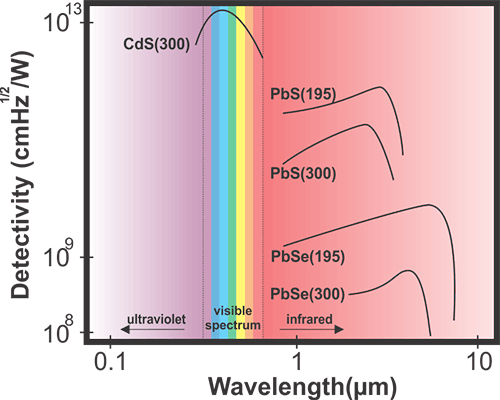
\includegraphics[width=0.6\linewidth]{imgs/wavelength-detectivity.png}
        \caption{Sensibilidade de LDR's de diferentes materiais face ao comprimento de onda}
        \label{fig:wavelenght}
    \end{figure}

Estas foto-resistências têm uma sensibilidade mais baixa que os foto-díodos e foto-transístores. Estes são semicondutores, usam a luz para controlar a passagem de electrões pelas lacunas da junção PN, enquanto os LDR's são componentes passivos, sem esta junção. Se a intensidade da luz for constante, a resistência pode variar ainda assim significativamente devido ás variações de temperatura, são também sensíveis a estas, fazendo com que os LDR's não sejam dispositivos de precisão.\\
\par Uma outra propriedade dos LDR's é que existe um atraso temporal entre as varições de luz e resistência, chamado de "\textit{resistance recovery rate}". Leva aproximadamente cerca de 10ms para a resistência diminuir assim que a luz é exposta depois de total escuridão. Ambiguamente, pode levar até 1s para o processo contrário. Por esta razão o LDR não pode ser usado onde as rápidas taxas de variação de luz existem e necessitam de ser registadas para actuação de dispositivos de controlo.\\
\par Neste trabalho os LDR's são implementados como básicos sensores de luz. Um circuito como o da figura [\ref{fig:ldr_circ}] pode ser implementado. O LED acende quando a intensidade da luz incidida sobre o LDR é suficiente. O potenciómetro é usado para estabelecer o limite em que queremos accionar o transistor. Se por sua vez, quisermos um sensor de escuridão, onde o LED acenderia na ausência de luz, bastava trocar o LDR e as duas resistências de posição.



\begin{figure}[H]
        \centering
        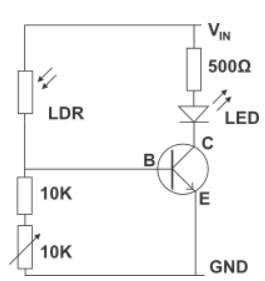
\includegraphics[width=0.4\linewidth]{imgs/LDR_circuit.png}
        \caption{Circuito de um LDR}
        \label{fig:ldr_circ}
    \end{figure}

%%%%%%%%%%%%%%%%%%%%%%%%%%%%%%%%%%%%%%%%%%%%%%%%%%%%%%%%%%%%%%%%%%%%%%%%%%%%%%%%%%%%%%%%%%%%%%%%%%%%

\subsubsection{Sensor de Humidade}
\par A humidade representa a quantidade de vapor de água presente no ar. Normalmente ínvisivel ao olho Humano, é indicada por precipitação, nevoeiro ou orvalho. A quantidade de vapor de água presente no ar para alcançar a saturação é maior consoante a temperatura. Esta quantidade de vapor de água presente num bloco de ar pode variar tanto que, por exemplo, um bloco de ar saturado, pode conter 28$g/m^3$ de ar a 40ºC, mas apenas 8$g/m^3$ a 8ºC.\\
\par As principais medidades de humidade normalmente utilizadas são: a absoluta, relativa e específica. \\
A húmidade absoluta quantifica a água presente no ar, e é descrita por $g/m^3$. Não tem a temperatura na sua equação, e na atmosfera toma valores desde próximos a 0 até ás 30$g/m^3$, quando o ar se encontra saturado a 30ºC. Representa então, a massa de vapor de água ($m_{H_2O}$) divida por um volume onde se encontra o bloco de ar ($V_{net}$).

\begin{equation}
    AH = \frac{m_{agua}}{V_{net}}
\end{equation}

A humidade relativa é uma medida importante, muito usada em previsões meteorológicas, é um indicador de precipitação, orvalho ou nevoeiro. Traduz também o "\textit{real-feel}" da temperatura, um aumento da humidade relativa significa uma maior sensação quer de frio, quer de calor, de acordo com o HeatIndex$^{\cite{heatindex}}$, uma humidade relativa de 75$\%$ a uma temperatura de 26ºC representaria uma sensação de 28ºC ($\pm$0.7ºC).\\
\par É expressa em percentagem, quanto maior o seu valor, mais húmido o ar se encontra. É definida pelo rácio da pressão parcial do vapor de água ($P_{H_2O}$) pelo equílibrio da pressão do vapor na água sobre uma superfície lisa de água pura a uma determinada temperatura ($P^*_{H_2O}$).

\begin{equation}
    RH (\phi) = \frac{P_{H_2O}}{P^*_{H_2O}}
\end{equation}

A humidade específica ($q$), é o rácio de massa de vapor de água ($r_v$) para a massa total da mistura ar/água.

\begin{equation}
    q = \frac{r_v}{1 + r_v}
\end{equation}

\par Um sensor de humidade detectam alterações de currente eléctrica ou temperatura no ar. E existem três tipos diferentes: Capacitivos, resistivos e térmicos. Todos eles monitorizam mudanças na atmosfera para calcular a humidade no ar.\\
\par O sensor capacitivo mede a humidade relativa colocando uma tira fina de óxido metálico entre dois eléctrodos, alterando a capacidade eléctrica do óxido com a humidade relativa presente na atmosfera (figura \ref{fig:humid_capac}).\\
São lineares e têm intervalos de leitura de 0-100$\%$. A desvantagem é que necessitam de um circuito complexo e de uma calibração frequente. No entanto são implementados em medições de precisão e são um elemento comum na medição de processos atmosféricos. Devido ao seu intervalo de leitura, é frequentemente usado em medições sem uma compensação activa de temperatura.

\begin{figure}[H]
        \centering
        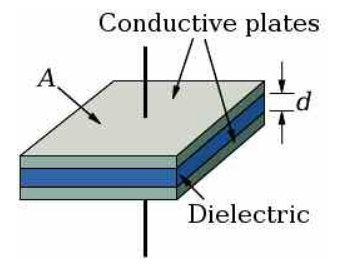
\includegraphics[width=0.4\linewidth]{imgs/capa_humid.png}
        \caption{Dieléctrico de sensor de humidade capacitivo}
        \label{fig:humid_capac}
\end{figure}

\par Sensores de humidade resistivos usam iões de sal para medir a impedância eléctrica dos átomos. Com o alterar da humidade, a resistência nos eléctrodos do objecto salínico também se altera.\\

Neste trabalho usámos o SHT21$^{\cite{SHT21}}$, com um sensor capacitivo, com sensor de temperatura em banda de lacuna e especializado em circuitos integrados analógicos e digitais, tudo isto em apenas um CMOS. Com um baixo consumo apresenta precisões de $\pm2\%$ de humidade relativa e $\pm$0.3ºC para a temperatura.

%%%%%%%%%%%%%%%%%%%%%%%%%%%%%%%%%%%%%%%%%%%%%%%%%%%%%%%%%%%%%%%%%%%%%%%%%%%%%%%%%%%%%%%%%%%%%%%%%%%%

\subsubsection{ESP8622}

\par Para efectuar a comunicação entre os sensores e o servidor é usado um ESP8622$^{\cite{arduino}}$ representado na figura [\ref{fig:8622}] para enviar os dados para o servidor. Este módulo é um microchip de baixo custo, com comunicações over-the-air por WiFi e usa o protocolo TCP/IP. Este ESP é o módulo sensorial para o sistema, recebe informação dos sensores e envia para a Raspberry através de MQTT$^{\cite{mqtt}}$.\\
Para integração da ESP8622 com a Arduino IDE$^{\cite{tuto}}$ foi usada uma biblioteca adicional, PubSubClient$^{\cite{pubsub}}$.

\begin{figure}[H]
        \centering
        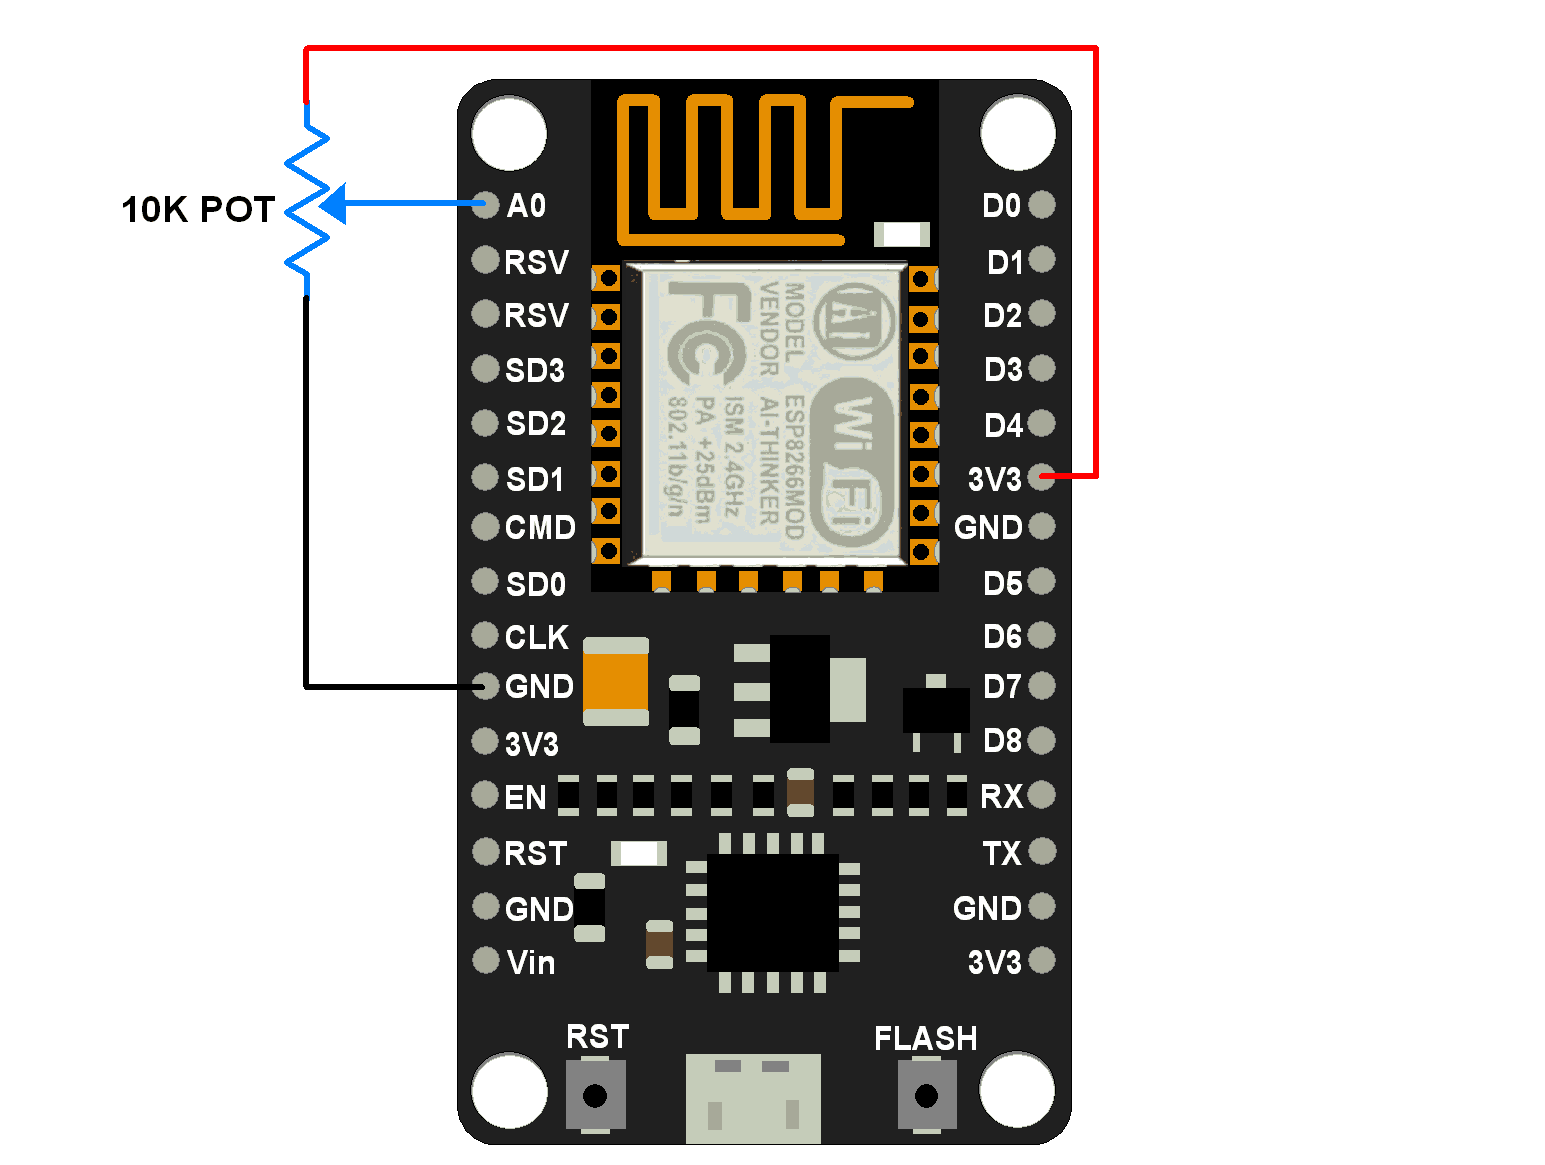
\includegraphics[width=0.4\linewidth]{imgs/NodeMCU_Potentiometer_Interface.png}
        \caption{ESP8622}
        \label{fig:8622}
\end{figure}
Este tambem comunica com o sensor SHT21 atraves do protocolo I2C
\begin{figure}[H]
        \centering
        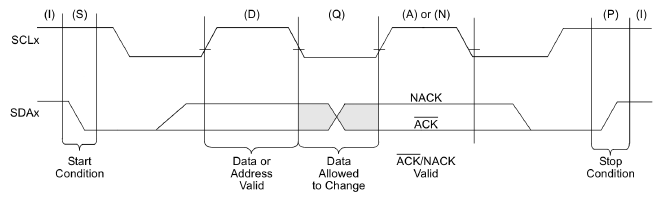
\includegraphics[width=0.7\linewidth]{imgs/I2C_time_diagram.png}
        \caption{Diagrama temporal protocolo I2C.}
        \label{fig:i2c_time}
\end{figure}
\begin{figure}[H]
        \centering
        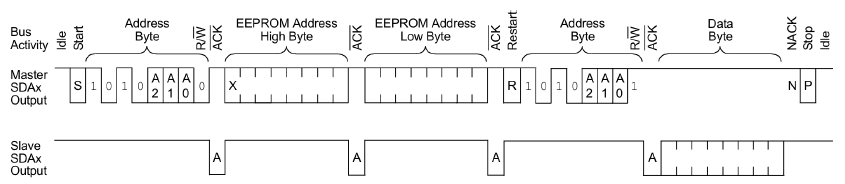
\includegraphics[width=0.7\linewidth]{imgs/I2C_data_transfer.png}
        \caption{Transferencia de dados entre um mestre I2C e uma memória.}
        \label{fig:i2c_transfer}
\end{figure}
Que funciona da seguinte forma:

\begin{enumerate}
    \item O dispositivo mestre inicia a comunicação com o Start-Bit
    \item O dispositivo mestre escreve o endereçco do dispositivo escravo (7 bits)
    \item O dispositivo mestre escreve o 8o bit de RW
    \item O dispositivo escravo escreve o sinal de ACK (Acknowledge)
    \item O dispositivo mestre (ou escravo) envia pacotes de 8 bits de dados, sempre seguidos
de um sinal ACK enviado pelo dispositivo escravo (ou mestre), confirmando a recepção
    \item O dispositivo mestre encerra a comunicação com o Stop-Bit
\end{enumerate}


É importante salientar as seguintes propriedades da comunicação I2C:
 O endereçamento por defeito é de 7 bits, mas existe o modo estendido de 10
bits.
 A quantidade de pacotes de transmissão é controlada pelo mestre e não existe
um valor máximo definido. Este é um ponto importante a ser tido em conta
quando se utilizam memórias uma vez que não existem os limites físicos de
endereçamento que existem nos dispositivos com interface paralelo.


\subsubsection{Raspberry PI, Mosquitto e NodeRed}

Como servidor do projecto, é usada uma Raspberry PI$^{\cite{rpi}}$ (figura [\ref{fig:rpi}]) ligada á mesma rede do ESP8622.\\

\begin{figure}[H]
        \centering
        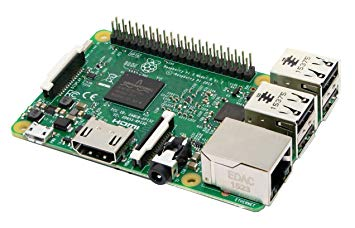
\includegraphics[width=0.4\linewidth]{imgs/raspberry.jpg}
        \caption{Raspberry PI}
        \label{fig:rpi}
\end{figure}

Eclipse Mosquitto$^{\cite{mosquitto}}$ é um projecto \textit{open source}, intermediário de mensagens que implementa o protocolo MQTT (Message Queuing Telemetry Transport)$^{\cite{mqtt}}$. Este protocolo fornece um método leve e viável de transportar uma mensagem usando um modelo de publicação/subscritor (figura [\ref{fig:mqttesp}]. É usado para as mensagens na área de \textit{Internet of Things}, tal como sensores de baixa potência ou dispositivos móveis.

\begin{figure}[H]
        \centering
        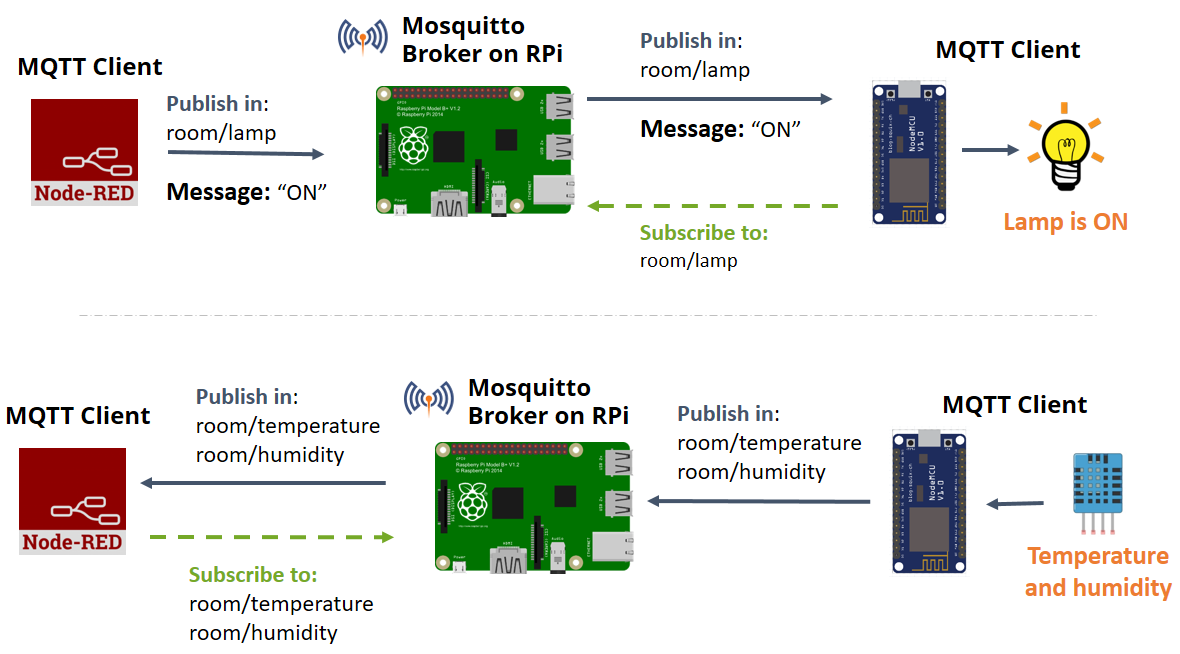
\includegraphics[width=0.8\linewidth]{imgs/MQTT-ESP8266-publish-and-subscribe-Node-RED.png}
        \caption{Publicação/Subscritor em MQTT com ESP8266}
        \label{fig:mqttesp}
\end{figure}

Com a finalidade de colocar toda a informação e a disponibilizar para uma página da rede, é usado o NodeRed$^{\cite{nodered}}$, uma ferramenta de programação em Node.js$^{\cite{nodejs}}$, que publica os dados na cloud, através de um editor embebido no \textit{browser} e, torna possível juntar o fluxo de informação num leque abrangente de nódulos na \textit{palette} (figura [\ref{fig:noderedpal}]).

\begin{figure}[H]
        \centering
        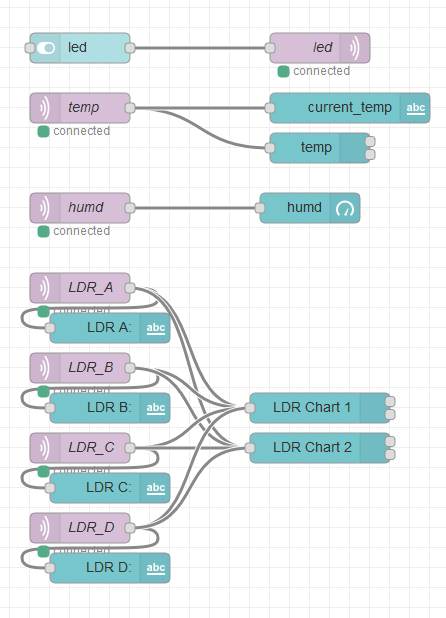
\includegraphics[width=0.4\linewidth]{imgs/SERVER_V04_NR_Code.png}
        \caption{Palette de nódulos do NodeRed}
        \label{fig:noderedpal}
\end{figure}

\subsubsection{PIC24FV16KM202}
\par Para adquirir os valores do sensor de luminosidade usamos a  PIC24$^{\cite{rpi}}$ (figura [\ref{fig:rpi}]) que depois envia estes valores para o ESP8622.\\

\begin{figure}[H]
        \centering
        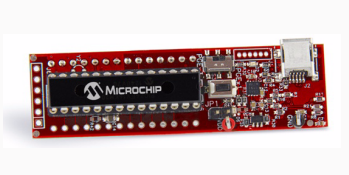
\includegraphics[width=0.4\linewidth]{imgs/PIC24.png}
        \caption{PIC24}
        \label{fig:pic24}
\end{figure}

A conversão de valores analógicos para digitais é fulcral. Os sensores recolhem valores analógicos, e os sistemas embebidos encarregues de os processar trabalham apenas com digitais. Assim estes sinais analógicos necessitam de ser convertido em digitais antes de serem enviados para a Raspberry neste caso. 

\begin{figure}[H]
        \centering
        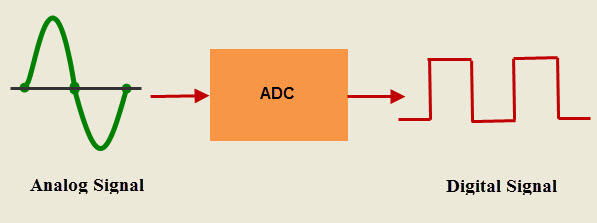
\includegraphics[width=0.4\linewidth]{imgs/ADC-Conversion.jpg}
        \caption{Conversão ADC}
        \label{fig:adc}
\end{figure}

\par O detalhe mais importante nesta conversão é a resolução do ADC. As resoluções mais comuns dísponiveis no mercado são de 8-bit, 10-bit e 12-bit. Por exemplo, se a tensão de referência da conversão A/D é de 0-5V, então um conversor A/D de 8-bit de resolução representa esta tensão num número, em 256 partes. Então consegue calcular a tensão exactamento até $\frac{5}{256} = 19 mV$, aproximadamente. Por outro lado, um conversor A/D de 10-bit divide essa tensão em 1024 partes. Aumentando a sensibilidade da conversão, uma vez que o de 8-bit não consegue reagir a uma diferença entre 1-18mV. \\
\par Outro detalhe para ter em conta é a taxa de amostragem, que define o quão rápido consegue o ADC de receber leituras. A Microchip$^{\cite{microchip}}$ reclama que os ADC's dos microcontroladores PIC's conseguem atingir as 100 mil amostragens/segundo.

Para adquirir estes valores optamos por escolher usar um ADC de aproximações sucessivas (SAR),com 12bits em que
\begin{equation}
    Resolucao = \frac{GamaValores}{2^n - 1} =\frac{5V}{2^(12) - 1} =1.22mV
\end{equation}
No trabalho anterior já tinhamos observado que a entrada do ADC é suscetível a ruido, como vemos na figura [\ref{fig:Hist_Noise_ADC}].\\

\begin{figure}[H]
        \centering
        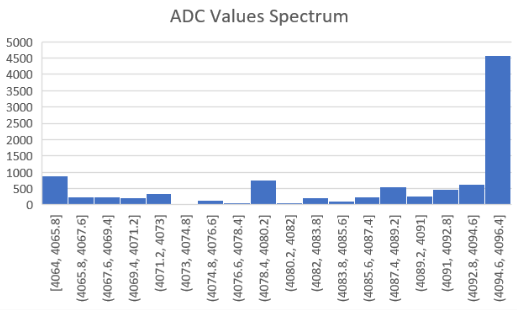
\includegraphics[width=0.4\linewidth]{imgs/Hist_Noise_ADC.png}
        \caption{Historama do Ruído à entrada do ADC}
        \label{fig:Hist_Noise_ADC}
\end{figure}
%%%%%%%%%%%%%%%%%%%%%%%%%%%%%%%%%%%%%%%%%%%%%%%%%%%%%%%%%%%%%%%%%%%%%%%%%%%%%%%%%%%%%%%%%%%%%%%%%%%%
\newpage
\section{Execução}
\par Começámos por adquirir os sinais de luminosidade através da PIC24$^{\cite{pic24}}$, para isso fizemos uso de 4 LDR's posicionados em cruz numa peça de plástico que desenhámos e imprimimos em 3D, como descrito na figura [\ref{fig:LDR_Matrix}].\\
Tendo os LDR's implementádo procedemos á calibração dos mesmos, para isso criámos um programa que apenas envia para o terminal os dados recebidos pela PIC em \textit{comma separated values (csv)} usamos este formato para depois processar os dados no Excel$^{\cite{excel}}$ e obter uma “recta” de calibração para cada LDR. Após esta calibração podemos obter o valor luminoso em cada LDR.
\textbf{Calibração dos LDR's}: Colocou-se uma fonte de luz directamente sobre a matriz dos LDR's, e fomos afastando a lampada para simular a diminuição de intensidade, verificando também os valores no sensor de luz embebido num telemóvel. Idealmente, este processo seria com uma lampada com reóstato e conseguiamos diminuir a intensidade sem alterar a posição da fonte luminosa. Então obtemos os valores para cada ADC pela porta série da PIC24 e colocámos no excel obtendo o gráfico da figura [\ref{fig:cal}].


\begin{figure}[H]
        \centering
        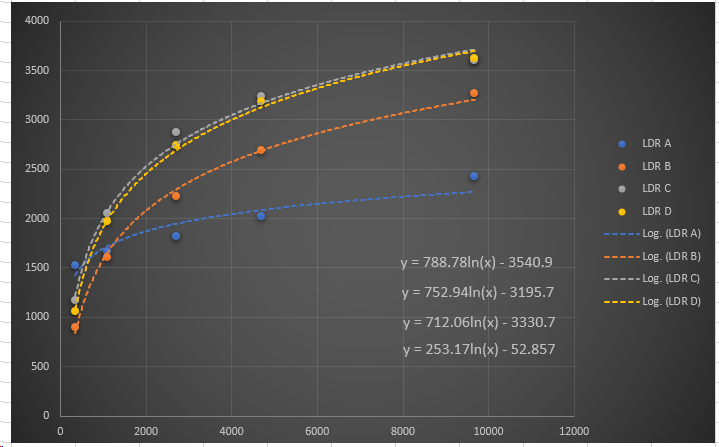
\includegraphics[width=0.7\linewidth]{imgs/ldrcal.png}
        \caption{Calibração}
        \label{fig:cal}
\end{figure}

\begin{figure}[H]
  \centering
  \begin{subfigure}[b]{0.5\linewidth}
    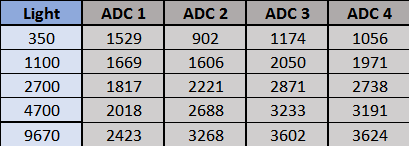
\includegraphics[width=\linewidth]{imgs/tabadc1.png}
    \caption{Resistência vs. Lux}
  \end{subfigure}
  \begin{subfigure}[b]{0.4\linewidth}
    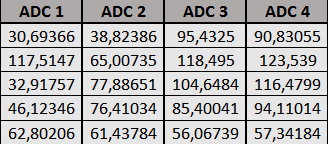
\includegraphics[width=\linewidth]{imgs/tabadc2.png}
    \caption{Desvio-Padrão}
  \end{subfigure}
  \caption{Tabelas de calibração dos LDR's}
  \label{fig:LDR_calib_tab}
\end{figure}

Após obter as equações das rectas, recorremos ao \textit{Matlab}$^{\cite{matlab}}$ para achar uma solução em ordem a \textbf{x} (figura [\ref{fig:matlab}]).

\begin{figure}[H]
        \centering
        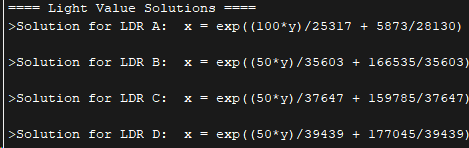
\includegraphics[width=0.7\linewidth]{imgs/matlab.png}
        \caption{Equações da recta de calibração}
        \label{fig:matlab}
\end{figure}

Então, usando um divisor de tensão para cada LDR conseguimos obter o valor da tensão no mesmo, ligando cada saída a um PIN analógico da PIC24, após implementação de um ADC conseguimos ler essa tensão.\\
Os valores após fazermos uma calibração conseguimos obter o valor da luz que incide no LDR.
Para isso implementamos 4 ADC's de 12 Bits, um para cada LDR, ligados aos Pinos AN0(2) AN1(3) AN2(4) AN3(5) respetivamente, agora fazendo uso do protocolo de comunicação UART conseguimos enviar os valores digitais adquiridos para o ESP8622, para isso basta ligarmos o PIN16(U1TX) da PIC ao pino RX do ESP8622.

\begin{figure}[H]
  \centering
  \begin{subfigure}[b]{0.31\linewidth}
    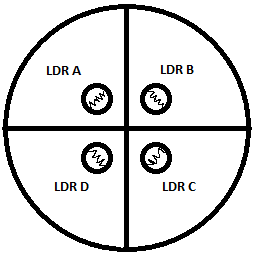
\includegraphics[width=\linewidth]{imgs/LDR_display_draft.png}
    \caption{Esquema}
  \end{subfigure}
  \begin{subfigure}[b]{0.3\linewidth}
    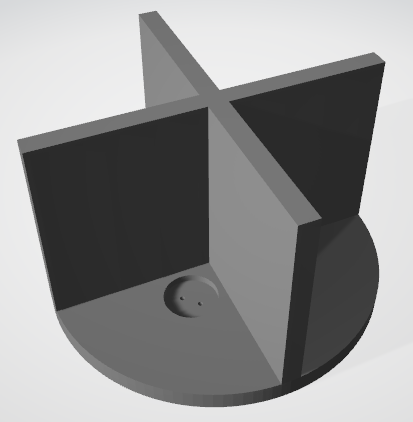
\includegraphics[width=\linewidth]{imgs/LDR_STAND_RENDER.png}
    \caption{3D Render}
  \end{subfigure}
  \begin{subfigure}[b]{0.3\linewidth}
    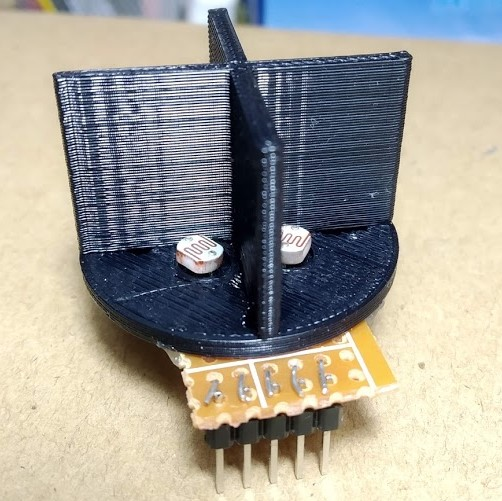
\includegraphics[width=\linewidth]{imgs/LDR_HUB_Foto.jpg}
    \caption{Sensor Final}
  \end{subfigure}
  \caption{Matriz de Photoresistencias}
  \label{fig:LDR_Matrix}
\end{figure}

Passando para o ESP8622, adquirimos os sinais da Humidade Relativa e da Temperatura do Sensor STH21, usando a biblioteca SparkFunHTU21D.h$^{\cite{spark_lib}}$ já implementada pela sparkfun, usando comunicação I2C com o ESP8622 ligamos o PIN SDA do Sensor ao PIN D2 e o SCL ao PIN D1 do ESP8622, tivemos de usar resistências de 220$\Omega$ em cada uma das linhas para conseguir comunicar.

\begin{figure}[H]
        \centering
        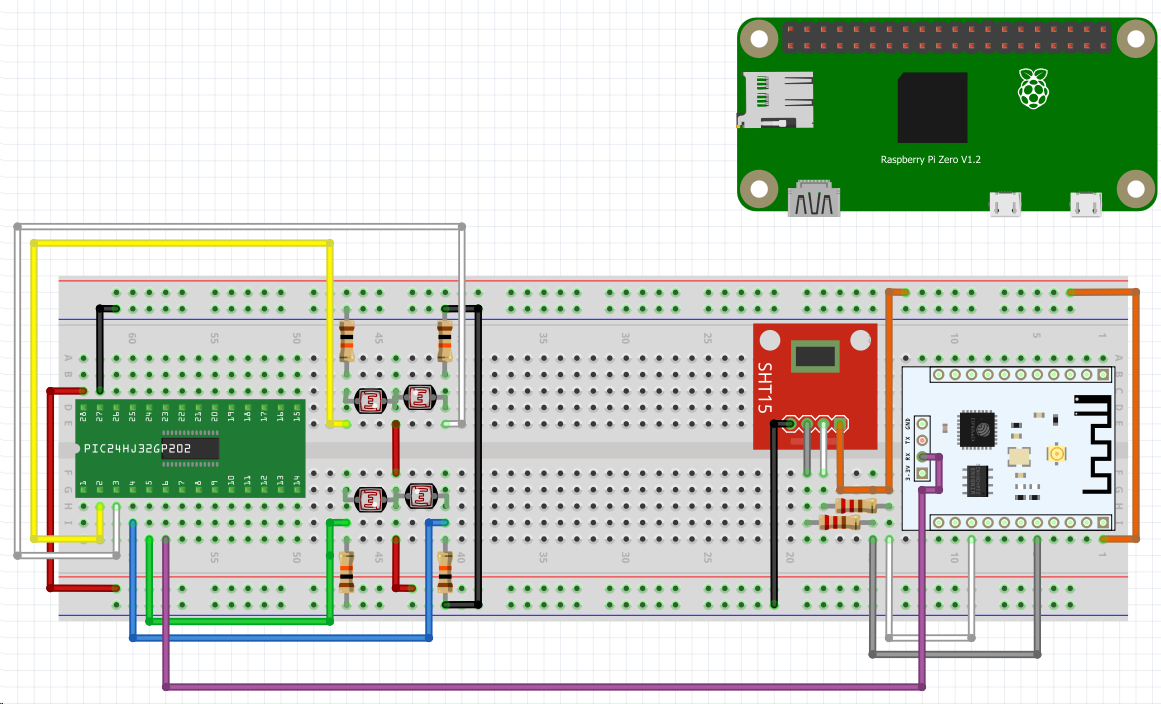
\includegraphics[width=0.7\linewidth]{imgs/circuit.png}
        \caption{Esquemático do circuito implementado na breadboard}
        \label{fig:circuit}
\end{figure}


Estamos agora prontos para enviar os dados para o nosso Agente de mensagens MQTT o Raspberry Pi, criando Tópicos para cada sensor.

\subsection{Guia de instalação}

Instalação do Mosquitto Client$^{\cite{mosquitto_install}}$
\begin{verbatim}
        sudo apt install -y mosquitto mosquitto-clients
        sudo systemctl enable mosquitto.service
\end{verbatim}

Instalação do Node Red$^{\cite{node_red_install}}$
\begin{verbatim}
        bash <(curl -sL https://raw.githubusercontent.com/node-red/raspbian-
            deb-package/master/resources/update-nodejs-and-nodered)	
        cd ~/.node-red
        npm i node-red-dashboard
        node-red-start
\end{verbatim}

\newpage
\section{Resultados}

Tendo agora toda a informação adquirida pelo nosso nódulo sensorial, resta apenas processá-la, para isso fizemos uso do NodeRed a correr no Raspberry Pi através do qual, subscrevendo aos tópicos enviados pelo nódulo sensorial (ESP8622) criámos uma página \textit{Web} que irá servir de interface do sistema e, por sua vez, apresentar os dados obtidos pelos sensores. Esta página \textit{Web} é facilmente acedida por todos os utilizadores presentes na rede local, situada no link 192.168.xx.xxx:1880/ui (figura [\ref{fig:Node_Red_Interface}]).

\begin{figure}[H]
  \centering
     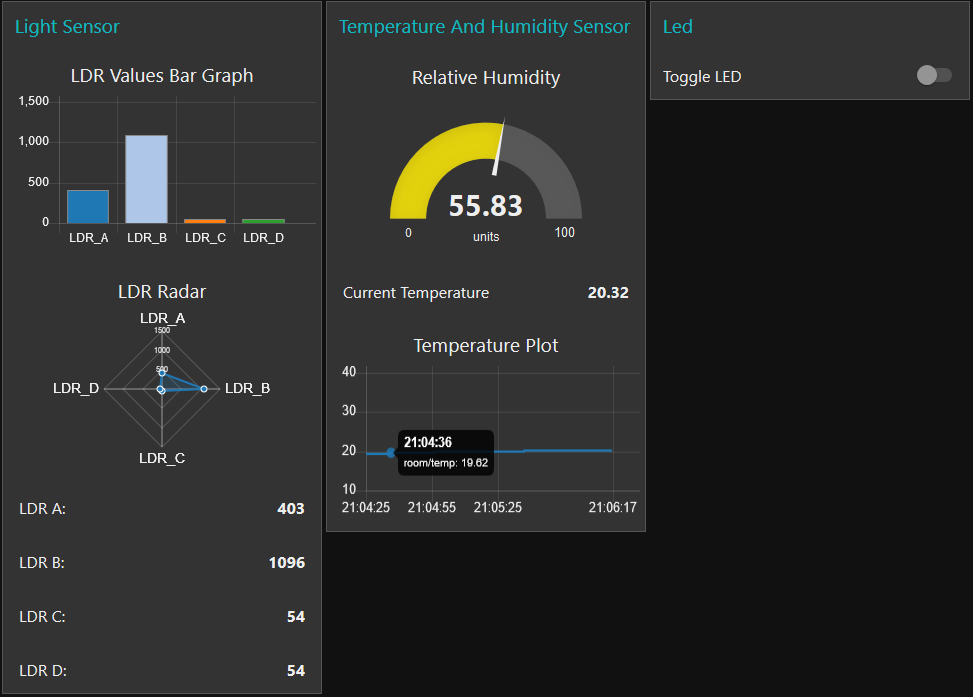
\includegraphics[width=0.7\linewidth]{imgs/SERVER_V04.png}
    \caption{Sensors Web-Page}
  \label{fig:Node_Red_Interface}
\end{figure}

\begin{figure}[H]
  \centering
     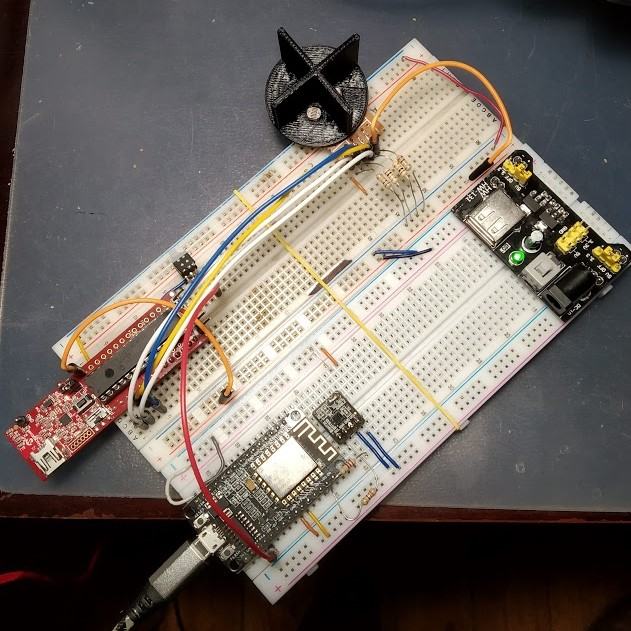
\includegraphics[width=0.7\linewidth]{imgs/V04_Physical_Circuit.jpg}
    \caption{Circuito Desenvolvido}
  \label{fig:physical_circuit}
\end{figure}

%%%%%%%%%%%%%%%%%%%%%%%%%%%%%%%%%%%%%%%%%%%%%%%%%%%%%%%%%%%%%%%%%%%%%%%%%%%%%%%%%%%%%%%%%%%%%%%%%%%%

\section{Conclusão}


A realização de um projecto de automação é sempre um desafio de engenharia: passar da ideia para o rascunho, do rascunho para o papel e do papel para a sua implementação. A utilização da raspberry PI como servidor externo para uma estação de sensores foi uma motivação extra, pois além de ser uma aplicação com um potencial enorme, é também de baixo custo, comparando com plataformas existentes actualmente. Se continuássemos com o desenvolvimento do trabalho, poderíamos implementar diferentes tipos de sensores, seja de gás ou até de água. Este projecto poderá ser integrado numa vastidade de áreas, tanto de controlo de ambiente local, accionando fontes de calor, ventilação ou de luminosidade, como simplesmente de monitorização e estudos ambientais, com a vantagem da comunicação MQTT entre o servidor e os seus sensores. 
Apesar das dificuldades, conseguimos atingir os objectivos, conseguindo assim monitorizar um ambiente fechado, obtendo os valores de luz temperatura e humidade relativa do mesmo.
A criação da matriz dos LDRs foi um desafio inexperado, embora se consiga lêr e obter uma boa ideia para qual dos sensores está a fonte de luz, a não lineareadade dos LDRs fez com que os nossos valores obtidos tivessem grande disparidade, podemos observar isto em expecifico no "LDR A" usado.
Após realização desta implementação ficamos com a noção do quão rápido é implementar um sensor obter valores e controlo do mesmo usando a internet of things.



\newpage

%%%%%%%%%%%%%%%%%%%%%%%%%%%%%%%%%%%%%%%%%%%%%%%%%%%%%%%%%%%%%%%%%%%%%%%%%%%%%%%%%%%%%%%%%%%%%%%%%%%%

\begin{thebibliography}{50}

\bibitem{libs}
\url{https://www.nedcc.org/free-resources/preservation-leaflets/2.-the-environment/2.1-temperature,-relative-humidity,-light,-and-air-quality-basic-guidelines-for-preservation}

\bibitem{green} 
\url{https://www.mas.bg.ac.rs/_media/istrazivanje/fme/vol42/2/11_nradojevic.pdf}

\bibitem{dry} 
\url{https://www.scs-usa.com/dry-rooms.html}

\bibitem{aqmesh} 
\url{https://www.aqmesh.com/wp-content/uploads/2018/07/AQMesh-technical-specification-V5.1-November-2018.pdf}

\bibitem{aeroqual} 
\url{https://www.aeroqual.com/product/sm70-fixed-gas-monitor}

\bibitem{BMP280} 
\url{https://cdn-shop.adafruit.com/datasheets/BST-BMP280-DS001-11.pdf}

\bibitem{hdc1080} 
\url{https://pt.mouser.com/new/Texas-Instruments/ti-hdc1080-sensor/}

\bibitem{no2sensor} 
\url{https://download.mikroe.com/documents/datasheets/110-502.pdf}

\bibitem{dustsensor} 
\url{https://www.sparkfun.com/datasheets/Sensors/gp2y1010au_e.pdf}

\bibitem{humidity} 
\url{https://en.wikipedia.org/wiki/Humidity}

\bibitem{resistor} 
\url{https://www.electronics-tutorials.ws/resistor/}

\bibitem{resistor} 
McGraw-Hill, Photodetection and Measurement - Maximizing Performance in Optical
Systems

\bibitem{heatindex} 
\url{https://en.wikipedia.org/wiki/Heat_Index}

\bibitem{humidity_sensor} 
\url{https://electronicsforu.com/resources/electronics-components/humidity-sensor-basic-usage-parameter}

\bibitem{SHT21} 
\url{http://www.farnell.com/datasheets/2307648.pdf}

\bibitem{spark_lib}
\url{https://github.com/sparkfun/SparkFun_HTU21D_Breakout_Arduino_Library}

\bibitem{arduino}
\url{https://www.arduino.cc/}

\bibitem{ESP8266}
\url{https://en.wikipedia.org/wiki/ESP8266}

\bibitem{node_red_install}
\url{https://nodered.org/docs/hardware/raspberrypi}

\bibitem{mosquitto_install}
\url{https://randomnerdtutorials.com/how-to-install-mosquitto-broker-on-raspberry-pi/}

\bibitem{rpi}
\url{https://www.raspberrypi.org/}

\bibitem{pubsub}
\url{https://pubsubclient.knolleary.net/ }

\bibitem{tuto}
\url{https://www.instructables.com/id/Steps-to-Setup-Arduino-IDE-for-NODEMCU-ESP8266-WiF/}

\bibitem{mqtt}
\url{https://en.wikipedia.org/wiki/MQTT/}

\bibitem{phys}
W. Smith e J.N. Cooper. Elements of
Physics

\bibitem{nodered}
\url{https://nodered.org/}

\bibitem{nodejs}
\url{https://nodejs.org/en/}

\bibitem{mosquitto}
W. Smith e J.N. Cooper. Elements of
Physics

\bibitem{pic24}
\url{http://www.farnell.com/datasheets/1509493.pdf}

\bibitem{excel}
\url{https://products.office.com/en/excel}

\bibitem{matlab}
\url{https://www.mathworks.com/products/matlab.html}

\bibitem{microchip}
\url{https://www.microchip.com/}



\end{thebibliography}


\end{document}